\documentclass[11pt,letterpaper,twocolumn]{article}
\usepackage{times}

\usepackage[utf8]{inputenc}
\usepackage[english]{babel}
\usepackage{float}
\usepackage{xcolor}
\usepackage{verbatim}
\usepackage{amsmath}
\usepackage{appendix}
\usepackage{ragged2e}
\usepackage{array}
\usepackage{etoolbox}
\usepackage{fancyhdr}
\usepackage{booktabs}
\usepackage{arydshln}
\usepackage{caption}
\usepackage{subcaption}
\usepackage{enumitem}
\usepackage{geometry}
\geometry{
  top=0.8in,            
  inner=0.5in,
  outer=0.5in,
  bottom=0.9in,
  headheight=4ex,       
  headsep=6.5ex,         
}
\usepackage{graphicx}
\usepackage{mathtools}
\usepackage{multirow}
\usepackage{pdfpages}
\usepackage{subfiles}
\usepackage[compact]{titlesec}
\usepackage{stfloats}
\usepackage[landscape, a4paper, margin=1in]{geometry} % page layout for half-page tables
\usepackage{hyperref}

\setlength{\columnsep}{30pt}


\pagestyle{fancy}
\fancyhf{}
      
\fancyfoot{}
\fancyfoot[C]{\thepage} % page
\renewcommand{\headrulewidth}{0mm} % headrule width
\renewcommand{\footrulewidth}{0mm} % footrule width

\makeatletter
\patchcmd{\headrule}{\hrule}{\color{black}\hrule}{}{} % headrule
\patchcmd{\footrule}{\hrule}{\color{black}\hrule}{}{} % footrule
\makeatother

\definecolor{blueM}{cmyk}{1.0,0.49,0.0,0.47}



\chead[C]{
      \begin{tabular}{m{1.5cm}m{11.5cm}m{2.5cm}}
      
\includegraphics[height=0.8cm]{imgs/um5 (1).png}
      &
      \centering
     \fcolorbox{white}{blueM}{\fbox{\begin{minipage}{11.5cm}
     \centering
     \textcolor{white}{ Mohammed V University}
     \end{minipage}}}
         &
        \centering
         \tiny{ \vspace{3.5mm} Faculty Of Sciences Rabat\\
%%%%%%%%%%%%%%%%%%%%%%%%%%%%%%%%%%%%%%%%%%%%%%%%%%%%%%%%%%%%%%%%%%%%%%%%%%%%%%%%%%%%%%%%%%%%%%%%%
          Submittion Date: 9/12/2024 \\ 
%%%%%%%%%%%%%%%%%%%%%%%%%%%%%%%%%%%%%%%%%%%%%%%%%%%%%%%%%%%%%%%%%%%%%%%%%%%%%%%
          }\tabularnewline
%          \hline
          \end{tabular}%
    }
    
\begin{document}
\twocolumn[\begin{@twocolumnfalse}


\begin{minipage}{0.15\textwidth}{
    
\includegraphics[width=4cm]{imgs/images (1).png }}
\end{minipage}
\hspace{25pt}
\begin{minipage}{0.75\textwidth}
\vspace{5mm}
    \Large{\textbf{Assignment 02: Image Filtering and Segmentation in MATLAB}} 
    \vspace{3mm}
    \par
    \textbf{Program: } Msc Intelligent Processing Systems\par
    \textbf{Course:} Computer Vision\par
    \textbf{Student:} El Mahraoui Amal \par
    \textbf{Lecturer:} El Hajoui Souhaila \par
    
    

\end{minipage}

\small

\vspace{11pt}

\centerline{\rule{0.95\textwidth}{0.4pt}}

\begin{center}
    
    \begin{minipage}{0.9\textwidth}
        % RESUMEN
        \noindent \textbf{Abstract:} This report presents an image processing task involving the filtering of noisy images using low-pass filters, followed by segmentation to isolate specific regions of interest. The images were subjected to Gaussian noise and Salt & Pepper noise, with the objective of comparing the effects of averaging and median filters of varying kernel sizes. The quality of the images was assessed using Mean Squared Error (MSE) and the Blind/Referenceless Image Spatial Quality Evaluator (BRISQUE). The segmentation task involved isolating the brighter regions of the noisy images using thresholding techniques. The results highlight the effectiveness of different filters in noise reduction and their impact on segmentation. 
    
        \vspace{4mm}
        % PALABRAS CLAVE
        \noindent \textbf{Key Words:} Image Filtering
Image Segmentation, Noise Reduction, MATLAB. 
    
    \end{minipage}
    
\end{center}

\centerline{\rule{0.95\textwidth}{0.4pt}}

\vspace{15pt}
\end{@twocolumnfalse}]
%%%%%%%%%%%%%%%%%%%%%%%%%%%%%%%%%%%%%%%%%%%%%%%%%%%%%%%%%%%%
\section{Introduction}
\justify
In the field of computer vision, image filtering and segmentation play a crucial role in improving image quality and isolating regions of interest for further analysis. Noise is often introduced during image acquisition, affecting the quality of the image and making subsequent analysis difficult. This report focuses on two types of image filtering—mean (averaging) and median filters—and their ability to remove Gaussian and Salt \& Pepper noise. Additionally, image segmentation techniques, such as global thresholding, were applied to segment out bright regions from the images. The impact of various filter sizes and segmentation methods on the final results was assessed.\par \vspace{5mm}  
%%%%%%%%%%%%%%%%%%%%

%%%%%%%%%%%%%%%%%%%%

%%%%%%%%%%%%%%%%%%%%%%%%%%%%%%%%%%%%%%%%%%%%%%%%%%%%%%%%%%%%
\section{Methodology}
\justify
\begin{enumerate}
    \item \textbf{Image Filtering}

The task involved filtering noisy images using two types of filters: the mean filter and the median filter. The images used were the original clean image "Ref.jpg", and two noisy images "m\_br1.jpg" (Gaussian noise) and "m\_br2.jpg" (Salt \& Pepper noise). For each filter type, different kernel sizes (3x3, 7x7, and 13x13) were applied. The following MATLAB functions were used:
\begin{itemize}
    \item \textbf{fspecial('average', kernel\_size)} to create the mean filter.\par
    \item \textbf{imfilter()} to apply the mean filter.\par
    \item \textbf{medfilt2()} to apply the median filter.\par
\end{itemize}


    \item \textbf{Image Quality Calculation}

The quality of the filtered images was evaluated using two metrics:

\begin{itemize}
    \item \textbf{Mean Squared Error (MSE):} This metric was calculated using the MATLAB function \textbf{immse()}, comparing the filtered images against the reference image.
    \item \textbf{BRISQUE:} The BRISQUE score was computed for each filtered image using the MATLAB \textbf{brisque() }function, which evaluates image quality without a reference.
\end{itemize}


\item \textbf{Image Segmentation} Segmentation was performed to isolate the brighter regions of the images. First, the histograms of the noisy images were visualized using \textbf{imhist()}. A global threshold was computed using \textbf{the graythresh()} function. The thresholding technique was applied both before and after filtering to evaluate the effect of filtering on segmentation. The best filtering method, based on subjective visual inspection, was selected for segmentation.
\end{enumerate}
%%%%%%%%%%%%%%%%%%%%%%%%%%%%%%%%%%%%%%%%%%%%%%%%%%%%%%%%%%%%
\section{Results}
\justify


\textbf{Filtering Results:}
% Insert two figures
\begin{figure}[H]
    \centering
    \begin{minipage}{0.45\textwidth}
        \centering
        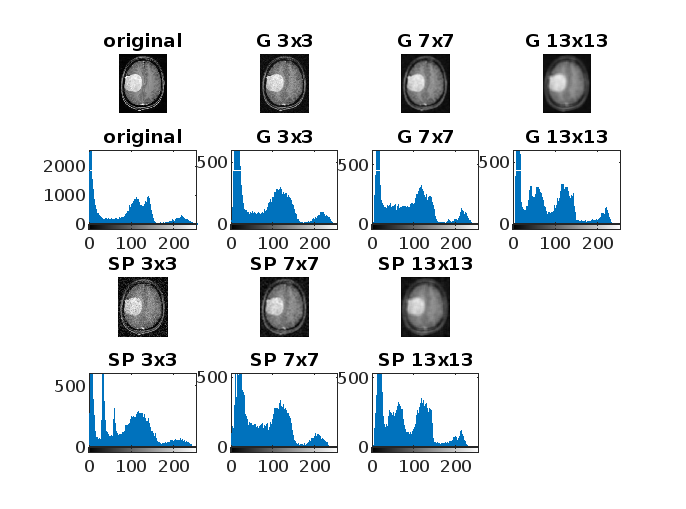
\includegraphics[width=\textwidth]{results/Figure 1.png}
        \caption{Filtered image with mean filter.}
        \label{fig:mean_filter_7x7}
    \end{minipage}\hfill
    \begin{minipage}{0.45\textwidth}
        \centering
        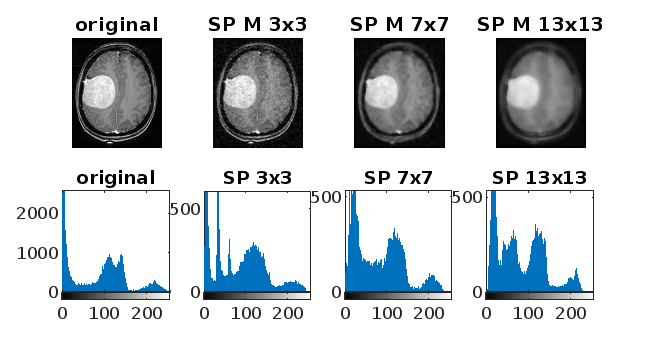
\includegraphics[width=\textwidth]{results/Figure 2.png}
        \caption{Filtered image with median filter.}
        \label{fig:median_filter_7x7}
    \end{minipage}
\end{figure}
The filtered images were obtained using the mean and median filters with kernel sizes of 3x3, 7x7, and 13x13. The images filtered with the median filter were generally better at removing Salt \& Pepper noise, whereas the mean filter was more effective in reducing Gaussian noise. Larger kernel sizes (13x13) generally provided smoother results but also introduced some blurring, as shown in the figure [\ref{fig:mean_filter_7x7}] and [\ref{fig:median_filter_7x7}].\par
\textbf{Histogram Analysis:} Histograms of the original and filtered images were plotted, showing how the distribution of pixel intensities changed after applying the filters. The median filter with a 7x7 kernel showed the best preservation of the image structure while effectively removing noise. \par \vspace{5mm}
\textbf{Quality Metrics:} The Mean Squared Error (MSE) values
for the filtered images were calculated and compared, as presented in the table below [\ref{tab:quality_metrics}]. Lower MSE values indicated better performance in terms of similarity to the reference image. The BRISQUE scores also suggested that the median filter with a 7x7 kernel performed best in terms of perceptual quality.\par \vspace{5mm}

%%%%%% Table 
\begin{table}[ht]
\centering
\small % Reduce the font size
\begin{tabular}{@{} l c c @{}} 
\toprule
\textbf{Condition} & \textbf{MSE} & \textbf{BRISQUE} \\ \midrule
\textbf{Without filter (br1)} & 2459.1565 & 43.4667 \\
\textbf{With mean filter (br1)} & 733.0191 & 48.6346 \\
\textbf{With median filter (br1)} & 576.8675 & 46.7624 \\ \midrule
\textbf{Without filter (br2)} & 574.7093 & 46.9084 \\
\textbf{With mean filter (br2)} & 660.3111 & 55.2497 \\
\textbf{With median filter (br2)} & 593.0471 & 44.1164 \\ \bottomrule
\end{tabular}
\caption{Quality metrics for different filters and noise types (br1 and br2).}
\label{tab:quality_metrics}
\end{table}
\textbf{Segmentation Results:} 
% Insert two figures
\begin{figure}[H]
    \centering
    \begin{minipage}{0.45\textwidth}
        \centering
        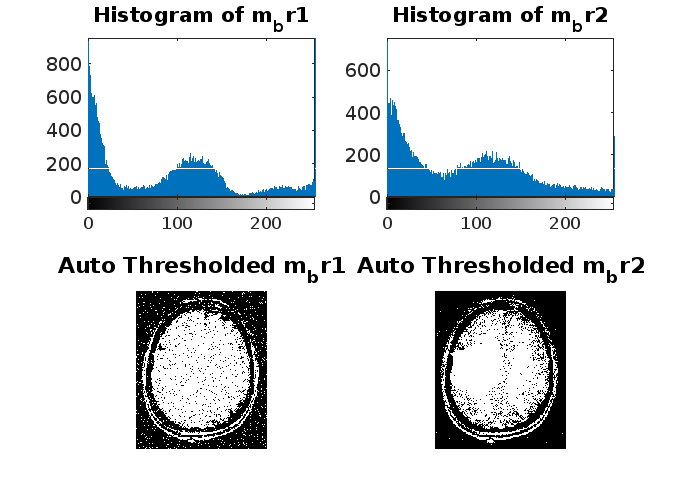
\includegraphics[width=\textwidth]{results/Figure 3.png}
        \caption{Filtered image with mean filter.}
        \label{fig:manual}
    \end{minipage}\hfill
    \begin{minipage}{0.45\textwidth}
        \centering
        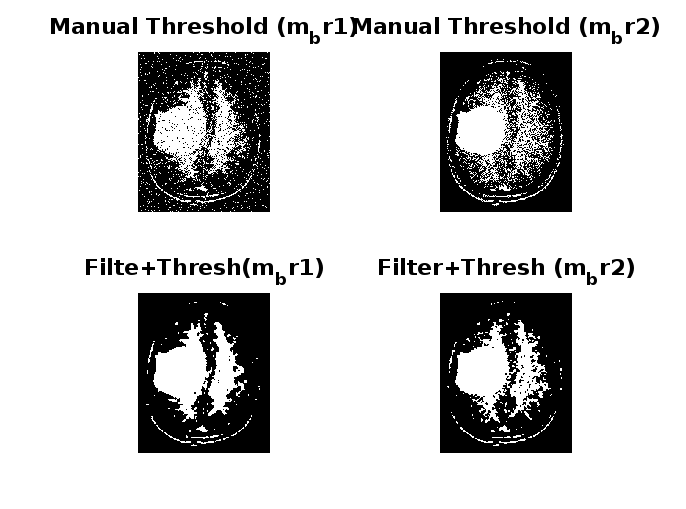
\includegraphics[width=\textwidth]{results/Figure 4.png}
        \caption{Filtered image with median filter.}
        \label{fig:auto}
    \end{minipage}
\end{figure}

Segmentation was successful in isolating the brighter regions of the images as illustrated in the figures below [\ref{fig:manual}]. The thresholding technique was effective in both noisy and filtered images, with the median filter providing better results in terms of accuracy [\ref{tab:segmentation_results}] and clarity (See figure [\ref{fig:auto}]) of the segmented areas.\par \vspace{5mm}

\begin{table}[ht]
\centering
\small % Reduce the font size for the table
\begin{tabular}{@{} l c @{}} 
\toprule
\textbf{Condition} & \textbf{Auto Threshold} \\ \midrule
\textbf{For m\_br1} & 0.32549 \\
\textbf{For m\_br2} & 0.33333 \\ \bottomrule
\end{tabular}
\caption{Manual \& Auto threshold values for segmentation of m\_br1 and m\_br2.}
\label{tab:segmentation_results}
\end{table}

%%%%%

\section{Discussion}
The filtering results showed that the median filter is more robust to Salt \& Pepper noise, while the mean filter is more effective against Gaussian noise. Larger kernel sizes, especially the 13x13 filter, led to more smoothing but also caused some loss of fine details. In terms of segmentation, the global thresholding technique worked well in separating the bright regions from the rest of the image, but it required careful selection of the threshold value, which varied depending on the noise level and filter applied.

The quality metrics, MSE and BRISQUE, provided insights into the effectiveness of the filtering techniques. The median filter with a 7x7 kernel achieved the best performance in both objective (MSE) and perceptual (BRISQUE) metrics, suggesting it is the most suitable for noise reduction in this context.
\section{Conclusion}
This study demonstrated the importance of filter selection and kernel size in both noise reduction and image segmentation tasks. Median filtering proved to be superior in handling Salt \& Pepper noise, while the mean filter was more effective for Gaussian noise. The segmentation results showed that filtering enhances the ability to isolate specific regions of interest in noisy images. The use of objective quality metrics such as MSE and BRISQUE was helpful in quantitatively assessing the performance of the filtering techniques. Future work could explore other filtering methods and their impact on segmentation, as well as fine-tuning the segmentation threshold for more accurate results.

\section{Appendix}
In this report, we have discussed the methodology and findings. The complete code used for these analyses can be found in the Appendix or on my [\href{https://github.com/aelmahraoui/MSc-IPS/tree/main/01.%201st%20semester/Computer%20Vision/Assignments/A02} {GitHub repository}].


%\section{Referencias}
 

\end{document}
